\documentclass[11pt, letterpaper]{article}

\usepackage{statcourse}
\usepackage{setspace}
\usepackage{times}
\usepackage{epsfig}
\usepackage{graphicx}
\usepackage{amsmath}
\usepackage{amssymb}
\usepackage{array,multirow}
\usepackage{url}
\usepackage{geometry}
\usepackage{threeparttable}
\usepackage{subfigure}

\geometry{letterpaper,left=2.54cm,right=2.54cm,top=.5cm,bottom=2.54cm}



% Include other packages here, before hyperref.

% If you comment hyperref and then uncomment it, you should delete
% egpaper.aux before re-running latex.  (Or just hit 'q' on the first latex
% run, let it finish, and you should be clear).
\usepackage[breaklinks=true,bookmarks=false]{hyperref}
\usepackage{cleveref}


\statcoursefinalcopy
\linespread{1.0}


%opening
\title{Body Fat Calculator}
\author{Hao Tong, Yuan Cao, Shushu Zhang}

\begin{document}


\maketitle

\section{Introduction}

Body fat is a highly specialized organ, critically important for health and longevity \cite{ludwig2016always}. It can be one of the most useful index for determining health and achieving fitness goal of an individual, even more than BMI. However, measurement techniques such as underwater weighing and air displacement plethysmography are always cumbersome to apply. Thus, it is meaningful to come up with a easier method to estimate the body fat with clinically available measurements. We are given a data set containing 252 observations whose body fat is accurately measuared and calculated by underwater weighing, together with 14 accessible predictors. 
%The report is organized as follows. Our rule is  

\section{Overall Findings \& Rule of Thumb}
\label{sec:2}
Regressed from the 14 predictors in the data set, "Bodyfat" can be estimated as
\begin{equation}\label{eq:model}
\begin{aligned}
\mathrm{Bodyfat}=
-28.81-0.13\mathrm{WEIGHT}-0.38\mathrm{NECK}+0.94\mathrm{ABDOMEN}+0.23\mathrm{BICEPS}\\
+0.41\mathrm{FOREARM}-1.14\mathrm{WRIST}.
\end{aligned}
\end{equation}
 
In this rule of thumb, the predictors are easily obtained in daily life. These six measurements are correlated to some extent. For example, one's abdomen circumference will typically increase as he gains weight. However, to obtain more accurate estimation of bodyfat, we typically need to know how much abdomen circumference has been increased per pound he gains. In the extreme case, if a men gains 1lb in weight but does not have any change in other variables sugguesting that he is building muscles instead of gaining fat, the model indicates that he will lose 0.13 in bodyfat. 


\section{Statistical Analysis}
To obtain the aforementioned rule of thumb, we need to first clean the data in \Cref{subsec:Cleaning}, and then fit a proper model in \Cref{subsec:model}. 
\subsection{Data Cleaning}
\label{subsec:Cleaning}
%It is natural to detect outliers by each variable seperately using techniques such as box plot. However, in data cleaning, we intend to impute the outliers that rise due to human errors instead of natural deviations in population distributions. In our case, the predictor variables have great redundancy (i.e. highly related). For example, ``ADIPOSITY", ``WEIGHT", and ``HEIGHT" are strictly related with the following equation 
%$$\mathrm{ADIPOSITY(bmi)} = \mathrm{BODY WEIGHT(kg)} : \mathrm{BODY HEIGHT(m^2)}.$$
%Anomalous observations that are supposed to be imputed or removed in advance, must have some inconsistency in different variables, while univariate outliers does not necessarily indicate anomalous observations. For example, observation No. 39 is way outlined in every variable, which will definitely be considered as an outlier if we consider variables seperately. However, it deviated in almost every variable at a similar degree, making it a reasonable observation of a highly overweight and obese person, thus the observation shouldn't been imputed. 

In order to detect the anomalous observations due to human errors instead of natural deviations in population distributions, we introduce \textbf{multivariate detections}, namely, fitting linear regressions for every variable with respect to other related variables using Residuals or Cook's Distance as a anomalous measure. Then, we concentrate on the extreme (maximum/minimum) values of each variable to make sure they make sense with practical meaning of the certain variable. To be more specific, in step 1, we fit ``DENSITY" with all other variables except ``IDNO" and ``BODYFAT" to make sure there is no obvious observation error in ``DENSITY". Then, we fit ``BODYFAT" with ``DENSITY", resulting in two outliers \emph{No. 48} and \emph{No. 96}. In addition, we detect an abnormal observation \emph{No. 42} by $\mathrm{ADIPOSITY(bmi)} = \mathrm{BODY WEIGHT(kg)} : \mathrm{BODY HEIGHT(m^2)}.$. Then, the rest of the variables are regressed similarly with all other variables except ``IDNO", resulting in anomalous observations of \emph{No. 31} and \emph{No. 86} for ``ANKLE", \emph{No. 175} for ``FOREARM". We impute all of the aforementioned anomalous observations with fitted values in the linear model or the defined equation. 
%We can even infer the error mechanisms for some imputations. No. 42, which has anomalously low value only in ``HEIGHT", can be imputed by the induced (or say redundent) variable ``ADIPOSITY" defined as 
%$\mathrm{ADIPOSITY(bmi)} = \mathrm{BODY WEIGHT(kg)} : \mathrm{BODY HEIGHT(m^2)}.$
%As a result, ``HEIGHT" OF No. 42, 29.50, is replaced by 69.45. 
%indicating 6 is probably mistyped by 2. Note that No. 163 and No. 221 also have slight mismatches in the relation of ``ADIPOSITY" with ``WEIGHT" and ``HEIGHT". But all three variables are in reasonable ranges, making it hard to determine the ``bad" observations. Therefore, we determine to leave as they are. 

In step 2, we use boxplot to detect the outliers in the target variable ``BODYFAT", resulting in finding the higher-end outlier \emph{No.216} and lower-end unreasonble point \emph{No. 182} with zero body fat. Owing to the uncertainty of the anomalous mechanism, we simply remove these two observations. 

\subsection{Model Selection}
\label{subsec:model}
In choosing the appropriate kind of model for handling this problem, linear regression outperforms several advanced machine learning models such as neural network in terms of both statistical accuracy and computational costs. For predictor selections, we use "olsrr:ols\_step\_best\_subset" function to obtain a subset of predictors that contribute to a large $R^2$ value with less variables. As a matter of fact, "abdomen" alone contributes to 0.63 $R^2$, making it the most important predictor among all, followed by "weight" variable. For better statistical accuracy, we finally use ``WEIGHT", ``NECK", ``ABDOMEN", ``BICEPS", ``FOREARM", ``WRIST" these six variables as predictors in linear regression model with $R^2$ 0.74, and other estimation and inference information listed in \Cref{tab:1}. 

\begin{table}[h!]
	\centering
	\caption{Estimated Coefficients}
	\resizebox{0.4\textwidth}{!}{
		\begin{tabular}{ccccccccccc}
			\hline\hline
&Estimate& Std. Error& t value &p value   \\
(Intercept)& -28.80735 &   7.13151 & -4.039& 7.17e-05 ***\\
WEIGHT  &     -0.12741  &  0.02557 & -4.982& 1.19e-06 ***\\
NECK    &     -0.37724  &  0.20620 & -1.829 & 0.06854 .  \\
ABDOMEN   &    0.93666 &   0.05212 & 17.971 & $<$ 2e-16 ***\\
BICEPS     &   0.22729  &  0.15156 &  1.500 & 0.13498    \\
FOREARM   &    0.40741 &   0.18000  & 2.263 & 0.02448 *  \\
WRIST    &    -1.14274 &   0.43254 & -2.642 & 0.00877 ** \\
			\hline
	\end{tabular}}
	\label{tab:1}
\end{table}


\section{Diagnostics}
\label{sec:diag}
For the linear model, we have the following assumptions: (1) observations are independent; (2) homoscedasticity; (3)linearity of the model; (4) error terms are normally distributed. The qq plot \Cref{fig:2} indicates that the residuals which are the estimations of error terms are approximately normally distributed. The standardized residual plot in \Cref{fig:2} suggests that the model is linear and homoscedastic, and there is no obvious outliers in the model, demonstrating the effectiveness of data cleaning. Based on Pii measure and Cook's distance in \Cref{fig:2}, we notice there are several leverage values and influence values, indicating there are points contributing to the model more than other points. However, they are not outliers. In conclusion, the assumptions of the model are satisfied. 
\begin{figure}
	\centering
	\label{fig:2}
	\begin{subfigure}
		\centering
		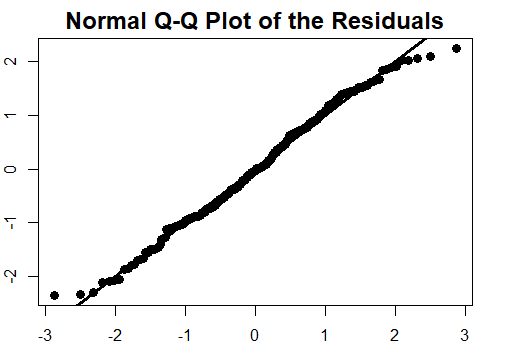
\includegraphics[width=.2\linewidth]{../Image/qq_plot.png}
	\end{subfigure}%
~
	\begin{subfigure}
		\centering
		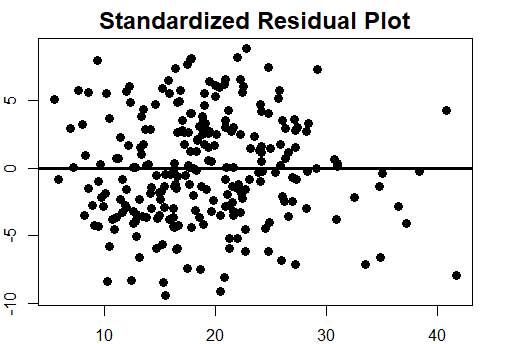
\includegraphics[width=.2\linewidth]{../Image/Final_Model_Residual_Plot.png}
	\end{subfigure}
	\begin{subfigure}
		%{.5\textwidth}
	\centering
	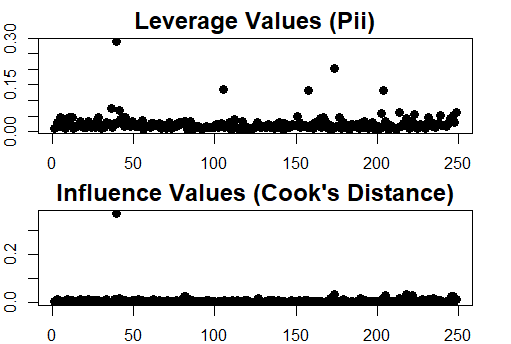
\includegraphics[width=.3\linewidth]{../Image/Pii_Cook's_Distance.png}
\end{subfigure}
	\caption{Diagnostics for Final Model}
\end{figure}
\section{Strengths and Weaknesses}
The strengths of our model lies in the interpretability, computation efficiency and predictability (i.e. statistical accuracy) as mentioned above. On the other hand, although the linearity assumption is approximately satisfied in \Cref{sec:diag}, these variables may not be linearly related to bodyfat in practice. 

\section{Conclusion}
As we come to a conclusion, we can use \Cref{eq:model} to calculate our body fat where abodomen circumference is the most importance predictor, followed by weight. 

\section{Contributions}
SZ:  \\
YC:   \\
HT:   \\

\pagebreak

{\small
\bibliographystyle{plain}
\bibliography{hungry.bib}
}



\end{document}
